\chapter{Исследовательская часть}

В данном разделе исследуется влияние наличия индекса на время выполнения запроса выборки данных из таблиц и объем дискового пространства, занимаемого хранимыми данными.

\section{Постановка исследования}

За основу выбирается функция добавления схемы (листинги~\ref{lst:add_chart_json:1}~--~\ref{lst:add_chart_json:2}). Для наглядности 

В листинге \ref{lst:idx} приведен запрос для создания индексов.

\begin{lstlisting}[label=lst:idx,caption=запрос для создания индексов]
    CREATE INDEX IF NOT EXISTS idx_branch_station_branch_id ON branch_station(branch_id);
    CREATE INDEX IF NOT EXISTS idx_station_title ON station(title);
    
    CREATE INDEX IF NOT EXISTS idx_branch_station_branch_id_station_id ON branch_station(branch_id, station_id);
    
    CREATE INDEX IF NOT EXISTS idx_branch_title ON branch(title);
    
    CREATE INDEX IF NOT EXISTS idx_chart_branch_chart_id ON chart_branch(chart_id);
    CREATE INDEX IF NOT EXISTS idx_chart_branch_branch_id ON chart_branch(branch_id);
    
    CREATE INDEX IF NOT EXISTS idx_branch_station_station_id ON branch_station(station_id);
    
    CREATE INDEX IF NOT EXISTS idx_station_transition_station_id ON station_transition(station_id);
    CREATE INDEX IF NOT EXISTS idx_station_transition_transition_id ON station_transition(transition_id);
    
    CREATE INDEX IF NOT EXISTS idx_railway_from_id ON railway(from_id);
    CREATE INDEX IF NOT EXISTS idx_railway_to_id ON railway(to_id);
    
    CREATE INDEX IF NOT EXISTS idx_chart_city ON chart(city);
    CREATE INDEX IF NOT EXISTS idx_chart_title ON chart(title);
    
    CREATE INDEX IF NOT EXISTS idx_station_occupancy ON station(occupancy);
    CREATE INDEX IF NOT EXISTS idx_station_open_time ON station(open_time);
    CREATE INDEX IF NOT EXISTS idx_station_close_time ON station(close_time);
    
    CREATE INDEX IF NOT EXISTS idx_transition_duration ON transition(duration);
    CREATE INDEX IF NOT EXISTS idx_transition_access ON transition(access);
    CREATE INDEX IF NOT EXISTS idx_transition_open_time ON transition(open_time);
    CREATE INDEX IF NOT EXISTS idx_transition_close_time ON transition(close_time);
\end{lstlisting}
Технические характеристики устройства, на котором выполнялись замеры времени:

\begin{itemize}
	\item операционная система --- Ubuntu 22.04.1 LTS Release: 22.04;
	\item оперативная память --- 16 ГБ, 3200 МГц;
	\item процессор --- AMD Ryzen 7 4800H with Radeon Graphics, 2900 МГц, ядер: 16.
\end{itemize}

\section{Результаты исследования}

\subsection{Скорость выполениня запросов}

На рисунке~\ref{chart:time} представлен график, иллюстрирующий зависимость времени выполнения запроса на выборку из таблицы схем от количества записей и от наличия индекса.

\begin{figure}[h]
    \centering
    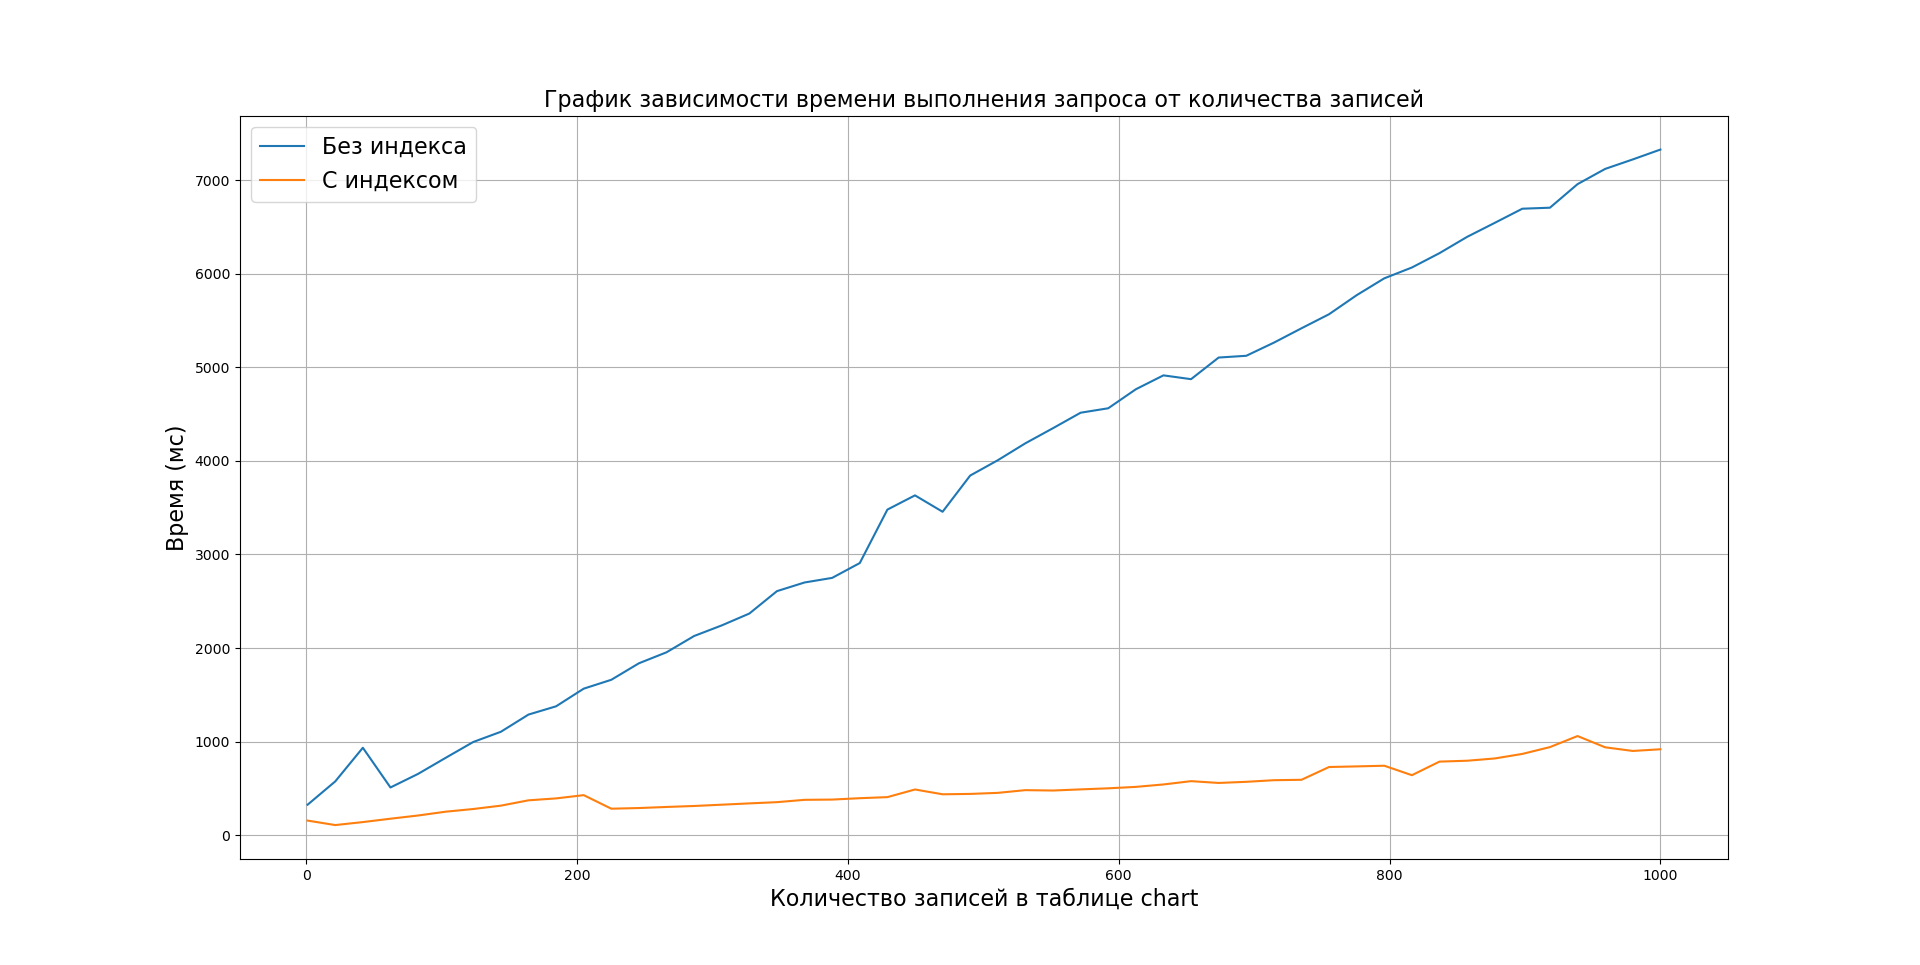
\includegraphics[width=\textwidth]{inc/img/Figure_1.png}
    \caption{График зависимости выполнения запроса от количества записей}
    \label{chart:time}
\end{figure}

% \imgScale{0.7}{time}{График зависимости времени выполнения запроса от объема данных}

\begin{table}[H]
    \centering
    \caption{Результаты замеров времени выполнения запросов}
    \label{tbl:query_time}
    \setlength{\tabcolsep}{4pt} % Уменьшаем отступы в ячейках
    \renewcommand{\arraystretch}{1.1} % Оптимальный межстрочный интервал
    \begin{tabular}{|r|r|r|}
        \hline
        \textbf{Кол-во записей} & \textbf{Без индекса (мс)} & \textbf{С индексом (мс)} \\
        \hline
        50 & 684 & 154 \\
        \hline
        100 & 796 & 241 \\
        \hline
        150 & 1\,118 & 332 \\
        \hline
        200 & 1\,499 & 419 \\
        \hline
        250 & 1\,837 & 301 \\
        \hline
        300 & 2\,196 & 323 \\
        \hline
        350 & 2\,626 & 355 \\
        \hline
        400 & 2\,847 & 382 \\
        \hline
        450 & 3\,630 & 463 \\
        \hline
        500 & 3\,932 & 456 \\
        \hline
        550 & 4\,356 & 477 \\
        \hline
        600 & 4\,597 & 505 \\
        \hline
        650 & 4\,868 & 657 \\
        \hline
        700 & 5\,167 & 572 \\
        \hline
        750 & 5\,548 & 722 \\
        \hline
        800 & 6\,005 & 634 \\
        \hline
        850 & 6\,370 & 790 \\
        \hline
        900 & 6\,628 & 842 \\
        \hline
        950 & 6\,953 & 946 \\
        \hline
        1000 & 7\,326 & 918 \\
        \hline
    \end{tabular}
\end{table}

Результаты показывают, что при увеличении количества записей в таблице с индексом время выполнения запроса практически не меняется, в то время как при отсутствии индекса наблюдается увеличение времени выполнения запроса.

\subsection{Использование дискового пространства}

Для определения занимаемого таблицами пространства использовалась функция PostgreSQL -- $pg\_total\_relation\_size$.

На рисунке~\ref{chart:size} представлен график зависимости объема дискового пространства от количества записей в таблице $chart$ при наличии и отсутствии индекса в базе данных.

\clearpage

\begin{figure}[h]
    \centering
    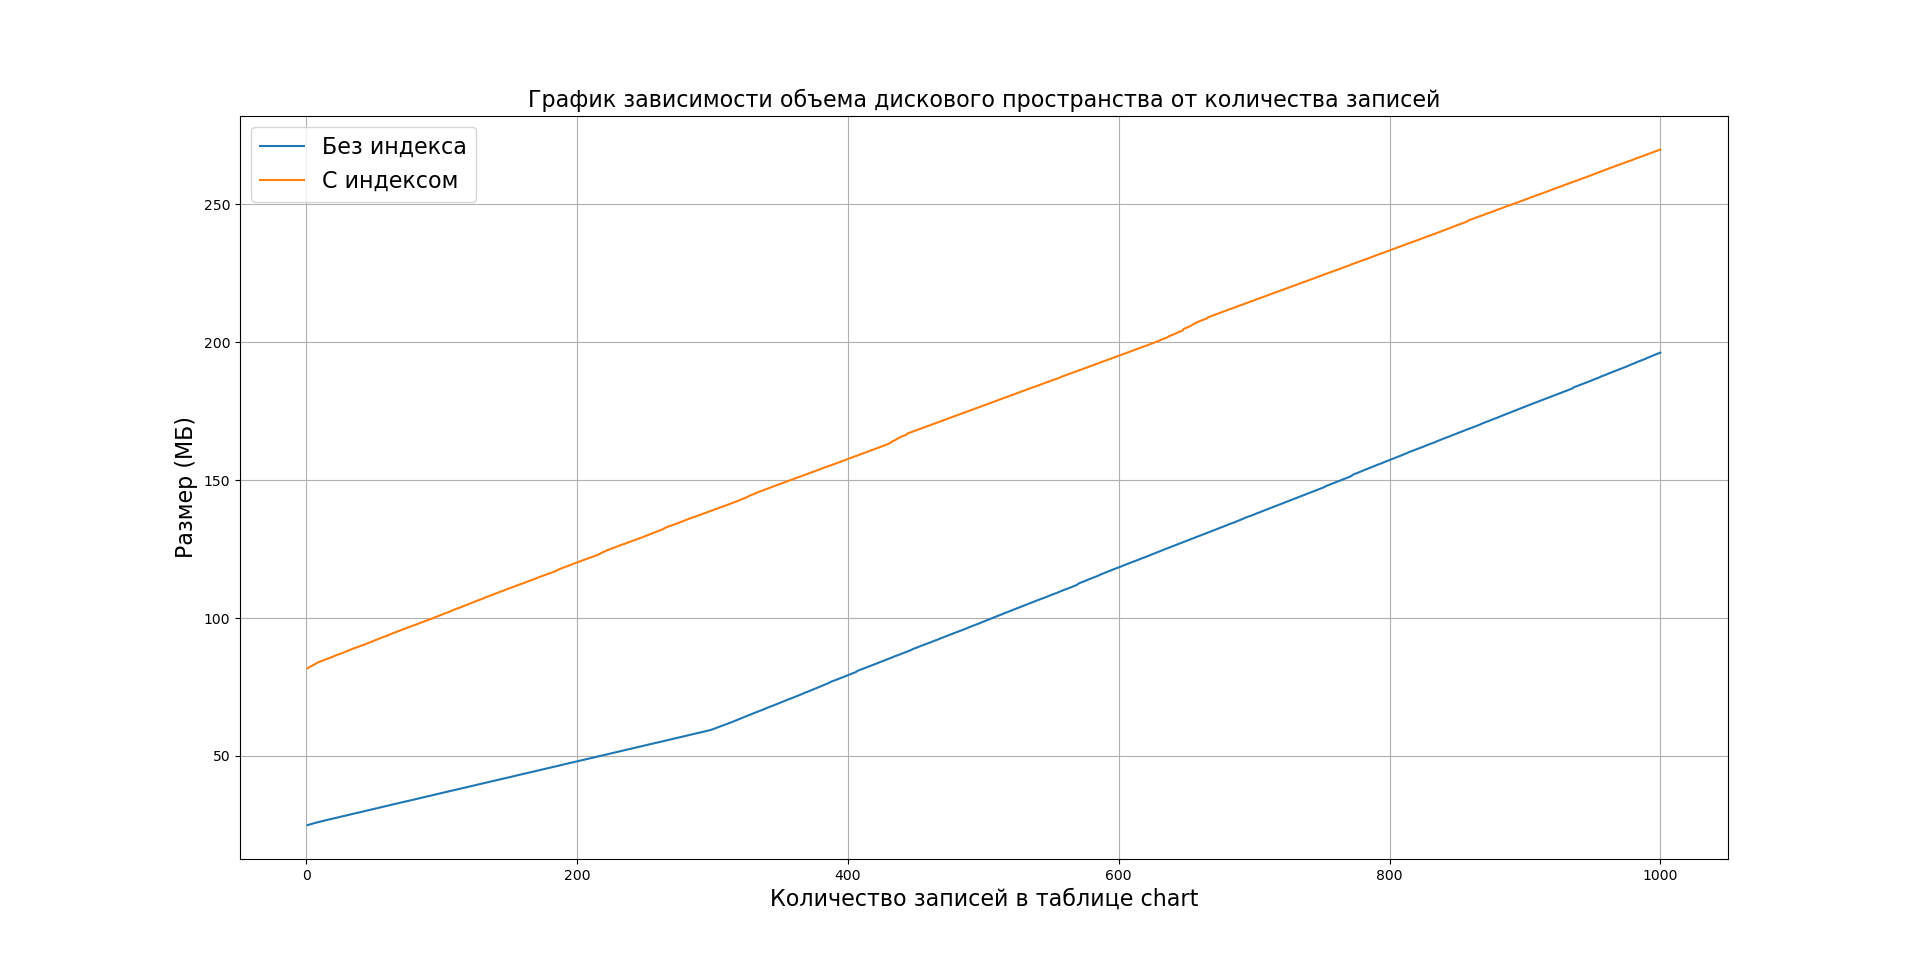
\includegraphics[width=\textwidth]{inc/img/Figure_2.png}
    \caption{График зависимости времени выполнения запроса от количества записей}
    \label{chart:size}
\end{figure}

\FloatBarrier

\clearpage

\begin{table}[H]
    \centering
    \caption{Результаты замеров объема занимаемой памяти}
    \label{tbl:query_time}
    \setlength{\tabcolsep}{4pt} % Уменьшаем отступы в ячейках
    \renewcommand{\arraystretch}{1.1} % Оптимальный межстрочный интервал
    \begin{tabular}{|r|r|r|}
        \hline
        \textbf{Кол-во записей} & \textbf{Без индекса (МБ)} & \textbf{С индексом (МБ)} \\
        \hline
        50 & 30.82 & 38.52 \\
        \hline
        100 & 36.58 & 45.72 \\
        \hline
        150 & 42.31 & 52.88 \\
        \hline
        200 & 48.05 & 60.06 \\
        \hline
        250 & 53.81 & 67.26 \\
        \hline
        300 & 59.66 & 74.57 \\
        \hline
        350 & 69.32 & 86.64 \\
        \hline
        400 & 79.29 & 99.11 \\
        \hline
        450 & 89.11 & 111.38 \\
        \hline
        500 & 98.66 & 123.32 \\
        \hline
        550 & 108.32 & 135.39 \\
        \hline
        600 & 118.34 & 147.92 \\
        \hline
        650 & 127.92 & 159.9 \\
        \hline
        700 & 137.53 & 171.91 \\
        \hline
        750 & 147.53 & 183.85 \\
        \hline
        800 & 157.25 & 196.56 \\
        \hline
        850 & 166.90 & 208.62 \\
        \hline
        900 & 176.57 & 220.71 \\
        \hline
        950 & 186.23 & 232.78 \\
        \hline
        1000 & 196.16 & 245.2 \\
        \hline
    \end{tabular}
\end{table}

\section*{Вывод}
Использование индексов позволяет оптимизировать время выполнения запроса к базе данных. Индексы занимают дополнительное дисковое пространство, но при это позволяют уменьшить время выполнения запроса. При максимальном количестве записей (1000) время выполнения запроса с использованием индексов уменьшилось более чем в 7 раз, в то время как занимаемое дисковое пространство увеличилось примерно на 25\%.
